%%%%%%%%%%%%
%
% $Autor: Wings $
% $Datum: 2019-03-05 08:03:15Z $
% $Pfad: ArduinoIDE.tex $
% $Version: 4250 $
% !TeX spellcheck = en_GB/de_DE
% !TeX encoding = utf8
% !TeX root = filename 
% !TeX TXS-program:bibliography = txs:///biber
%
%%%%%%%%%%%%



\chapter{Arduino IDE 1.8.x}\label{ArduinoIDE}



%%%%%%%%%%%%%%%%%%%%
\section{Introduction}

In this chapter we will be going through the description of the Arduino IDE and describe  the features of it and what are all the options present in the IDE and how can we use it. Further we will be describing about the installation procedure of the Arduino IDE and how to get started with it.

\section{Arduino IDE Description}

It is an open source official Arduino software which used for editing, uploading and compiling codes in to the Arduino module. It is a cross-platform software which is available for Operating Systems like Windows, Linux, macOS. It runs on Java platform and supports a range of Arduino modules. It supports C and C++ languages. The microcontrollers present on the Arduino boards are programmed which accepts the information in the form of code. The program written in the IDE is called a sketch which will generate a Hex file which is then transferred and uploaded in the controller. The IDE environment is made up of two parts: an editor and a compiler. The editor is used to write the required code, while the compiler is used to compile and upload the code to the Arduino Module.\cite{Fezari:2018}

The Menu bar has options such as File in which there are many options including Opening a new file or existing,  Examples-in which we can find sketches for different applications like Blink, Fade etc.  There is an error console at the bottom  of the screen for displaying errors.
 
\begin{figure}
	\centering
	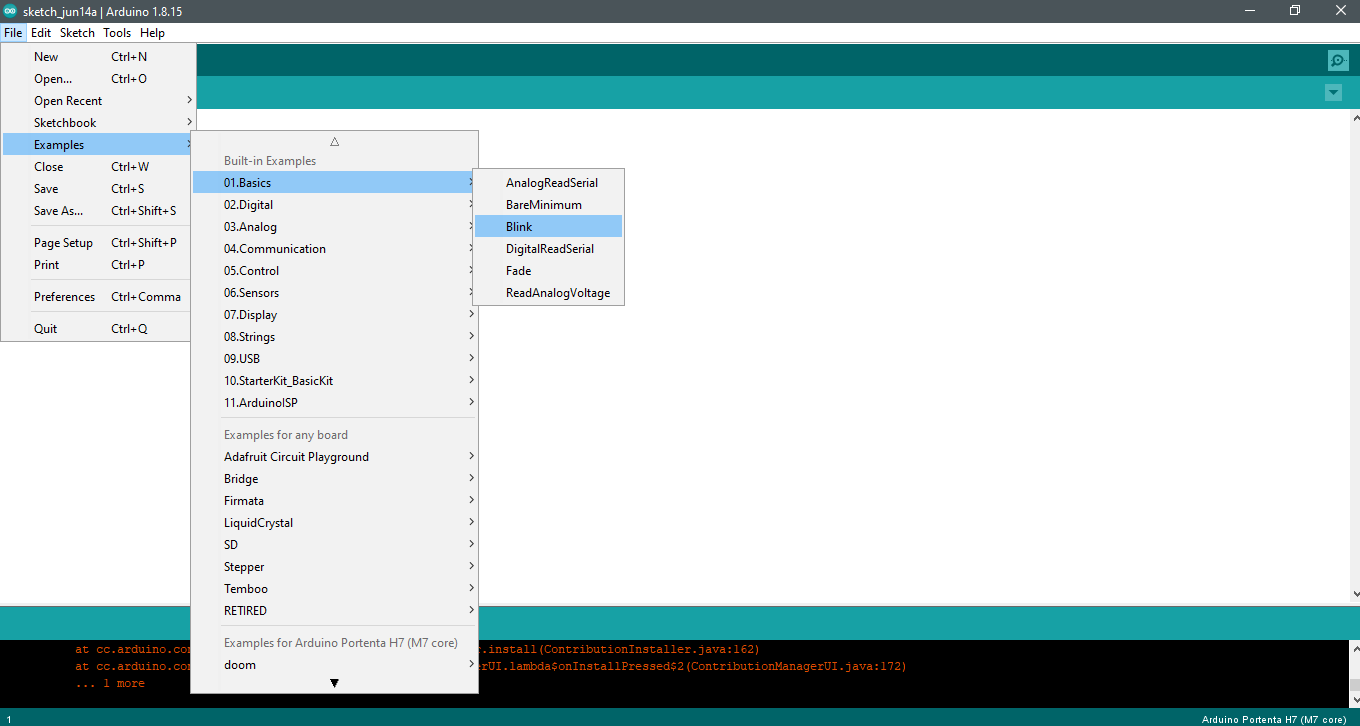
\includegraphics[width=0.9\textwidth]{Arduino/examplesketch}
	\caption{Menu bar options}\label{ArduinoIDEexamplesketch}
\end{figure}

The 6 buttons are present on top of the screen are presented in figure \ref{ArduinoIDEmenubar}.

\begin{figure}
	\centering
	
\includegraphics[width=0.9\textwidth]{Arduino/menubar}
	\caption{Menu butons}\label{ArduinoIDEmenubar}
\end{figure}

\begin{itemize}
	\item	The check mark is used to verify your code. Click this once you have written your code.
	\item	The arrow uploads your code to the Arduino to run.
	\item	The dotted paper will create a new file.
	\item	The upward arrow is used to open an existing Arduino project.
	\item	The downward arrow is used to save the current file.
	\item	The far right button is a serial monitor, which is useful for sending data from the Arduino to the PC for debugging purposes.
\end{itemize}


\section{Installation}

To install the Arduino IDE, we need to download the latest version from the Arduino webpage \url{https://www.arduino.cc/en/software}. We can select the version based on the operating system we are using. Here we are installing Arduino 1.8..15 for a Windows 10 operating system. 
The set up file name is arduino-1.8.15-windows.exe and the size of it is 1,17,470 KB. we can specify the path according to our needs. Here the path is set as  \SHELL{C:/Program Files (x86)/Arduino}. The most recent offline arduino IDE 1.8.15 can be seen in Figure, \ref{fig:arduino-creat-agent-installieren} it is also supportive for all operating systems.

\begin{figure}[h]
    \centering
    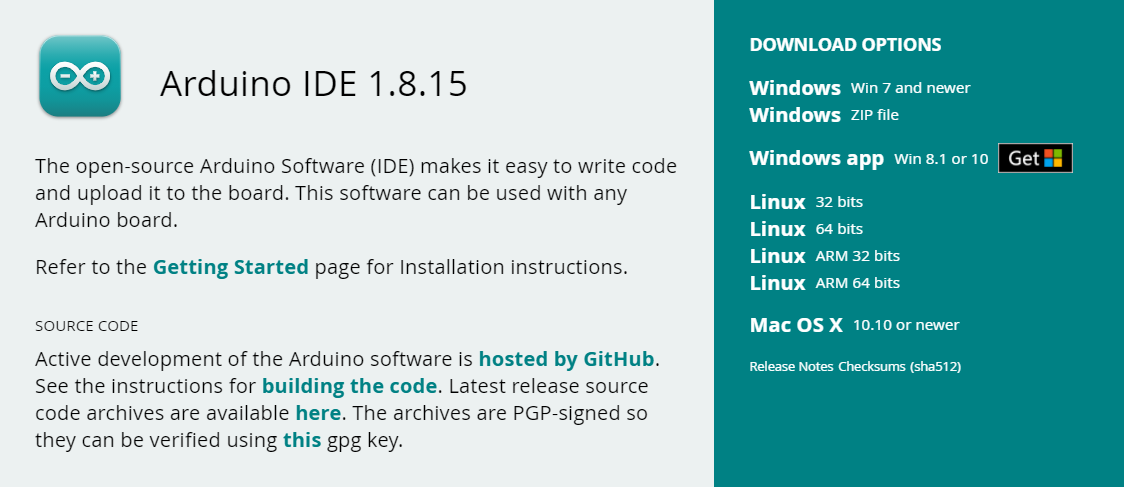
\includegraphics[width=1.0\linewidth]{Nano33BLESense/Installation-1}
    \caption{Arduino Creat Agent Installation}
    \label{fig:arduino-creat-agent-installieren}
\end{figure}

After the download is done, open the setup file and proceed to install.
Select all the components in the dialog box and click Next.

\begin{figure}
	\centering
	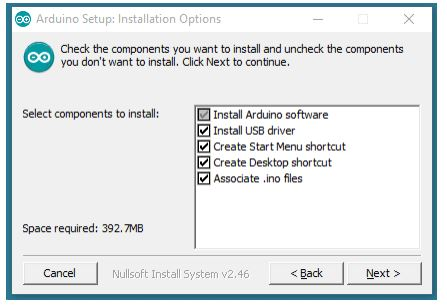
\includegraphics[width=0.7\textwidth]{Arduino/arduinoinst1}
	\caption{Arduino Setup Installation options}\label{ArduinoIDEInst1}
\end{figure}

Select the destination folder and click Install

\begin{figure}
	\centering
	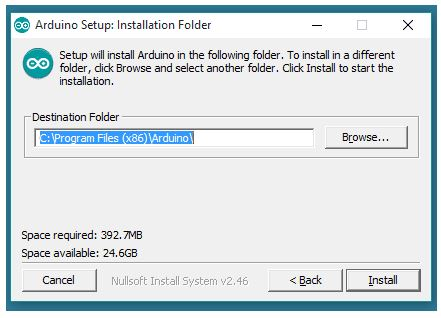
\includegraphics[width=0.7\textwidth]{Arduino/ardinst2}
	\caption{Arduino Setup: Installation Folder}\label{ArduinoIDEInst2}
\end{figure}

Once the installation is done, open the Arduino IDE and a default sketch appears on the screen as shown.

\begin{figure}
	\centering
	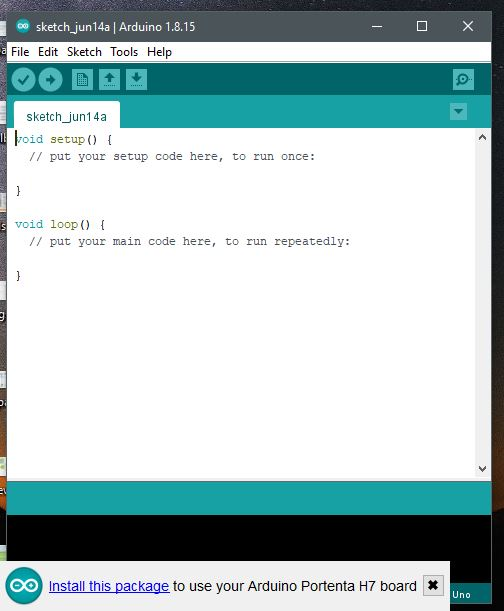
\includegraphics[width=0.7 \textwidth]{Arduino/arduinoidefrst}
	\caption{Arduino Sketch}\label{ArduinoIDEFirst}
\end{figure}

It can be seen from the figure \ref{ArduinoIDEFirst} that the basic arduino sketch has two parts. The first part is the function \PYTHON{void setup()} which returns void and we do the intiliaztion such as the output LED color, specifying the core etc. The second part is the function \PYTHON{void loop()} where we define functions which are to be performed through out the loop. These codes are placed between paranthesis \PYTHON{$\{ \}$} and each function has a return type, here it has void return type.


